%% This is an example first chapter.  You should put chapter/appendix that you
%% write into a separate file, and add a line \include{yourfilename} to
%% main.tex, where `yourfilename.tex' is the name of the chapter/appendix file.
%% You can process specific files by typing their names in at the 
%% \files=
%% prompt when you run the file main.tex through LaTeX.
\chapter{Evaluation}

With GERT, the programmer should be able to implement concurrent embedded programs
which are as performant as the equivalent C implementation, but without having to
worry about concurrency abstractions and memory safety bugs. In order to evaluate GERT,
there are two questions that must be answered:

\begin{enumerate}
  \item Does GERT retain good performance despite the costs of using a High Level Language?
  \item Do the concurrency patterns of Go simplify the task of the programmer?
\end{enumerate}

The first question is addressed by micro benchmarks which measure GERT's
speed in creating and responding to external events. Pin toggle (\ref{sec:pin_toggle})
measures the maximum pin toggle frequency. Response latency (\ref{sec:int_time})
measures the minimum time it takes to respond to an external interrupt. Event
throughput (\ref{sec:thruput}) measures the maximum number of total events that each platform
can reliably detect, as well as how this amount scales with additional CPU's monitoring
more simultaneous events.

%%Pulse counting
%%(\ref{sec:pulse_count}) counts number of pulses at increasing frequencies.
%%Concurrent response (\ref{sec:concurrency}) measures how many external events
%%GERT can concurrently respond to.

The second question is harder to answer because difficulty is a subjective
measure. This thesis attempts to show that GERT presents a better framework for
concurrency through two case studies: a robot sensor platform (\ref{sec:robot})
,which runs motors and reads sensors, and a galvo laser projector (\ref{sec:laser})
which traces images onto a surface by rotating mirrors at high speeds. The case studies
present a real-world experience for using GERT.

\section{Experimental Setup} \label{sec:setup}
In all tests, GERT is run on an i.MX6Quad SOC, which sits on a Wandboard
platform, and all measurements are taken
with a Rigol DS1054Z oscilloscope. When GERT is compared to Linux, the SOC
runs Debian 8 "Jessie" with hardfloat support. GERT is also occasionally
compared to a Teensy 3.2 microcontroller running C. The Teensy 3.2 uses a Cortex M4, which is specifically
intended for microcontroller applications, and has good real-time performance. Even though
the Cortex M4 has a vastly different architecture and purpose than the iMX6, its event
response times represent a good comparison point for GERT and Linux.
The Teensy platform
has poor concurrency support though because its Cortex M4 is a single core processor.
%%and it only has 64 kilobytes of RAM.

%%used
%%for the laser projector (\ref{sec:laser}).

%%GERT is evaluated in conditions that are representative of embedded workloads.
%%The first few tests are benchmarks which measure GERT's maximum interrupt
%%frequency and pin toggle rate. The last two tests are each case studies: a robot
%%sensor platform and a scanning-mirror galvanometer laser projector. The test SOC
%%is the Freescale i.MX6Quad. Depending on the test, it is either running assembly,
%%GERT, or Debian 8 "Jessie" with hardfloat support. A Teensy 3.2 is used for comparison
%%on a few of the latency tests because of its Cortex M4 processor. All timing
%%measurements are taken using a Rigol DS1054Z oscilloscope.

\section{Micro benchmarks}

\subsection{Pin Toggle Frequency}\label{sec:pin_toggle}
This test measures the speed at which GERT can toggle a simple GPIO pin on
the iMX6 Quad SOC. GPIO pins are an MMIO peripheral on the iMX6 which requires
many clock domain crossings to produce an output. After the toggle program sets
the state of a GPIO pin, this information must pass through the memory bus,
GPIO peripheral, and IO multiplexer peripheral before arriving to the output (\ref{fig:pipeline}).
The latency of this whole process is determined by the 66MHz peripheral clock,
which is the slowest clock in the pipeline. Therefore, the maximum frequency
of the square wave that can generated by the toggle program is approximately $\frac{\frac{66MHz}{3}}{2}=11MHz$. The presence
of additional pipeline stages inside the GPIO or IO multiplexer blocks will further
reduce this frequency.

\begin{figure}[h]
\begin{center}
  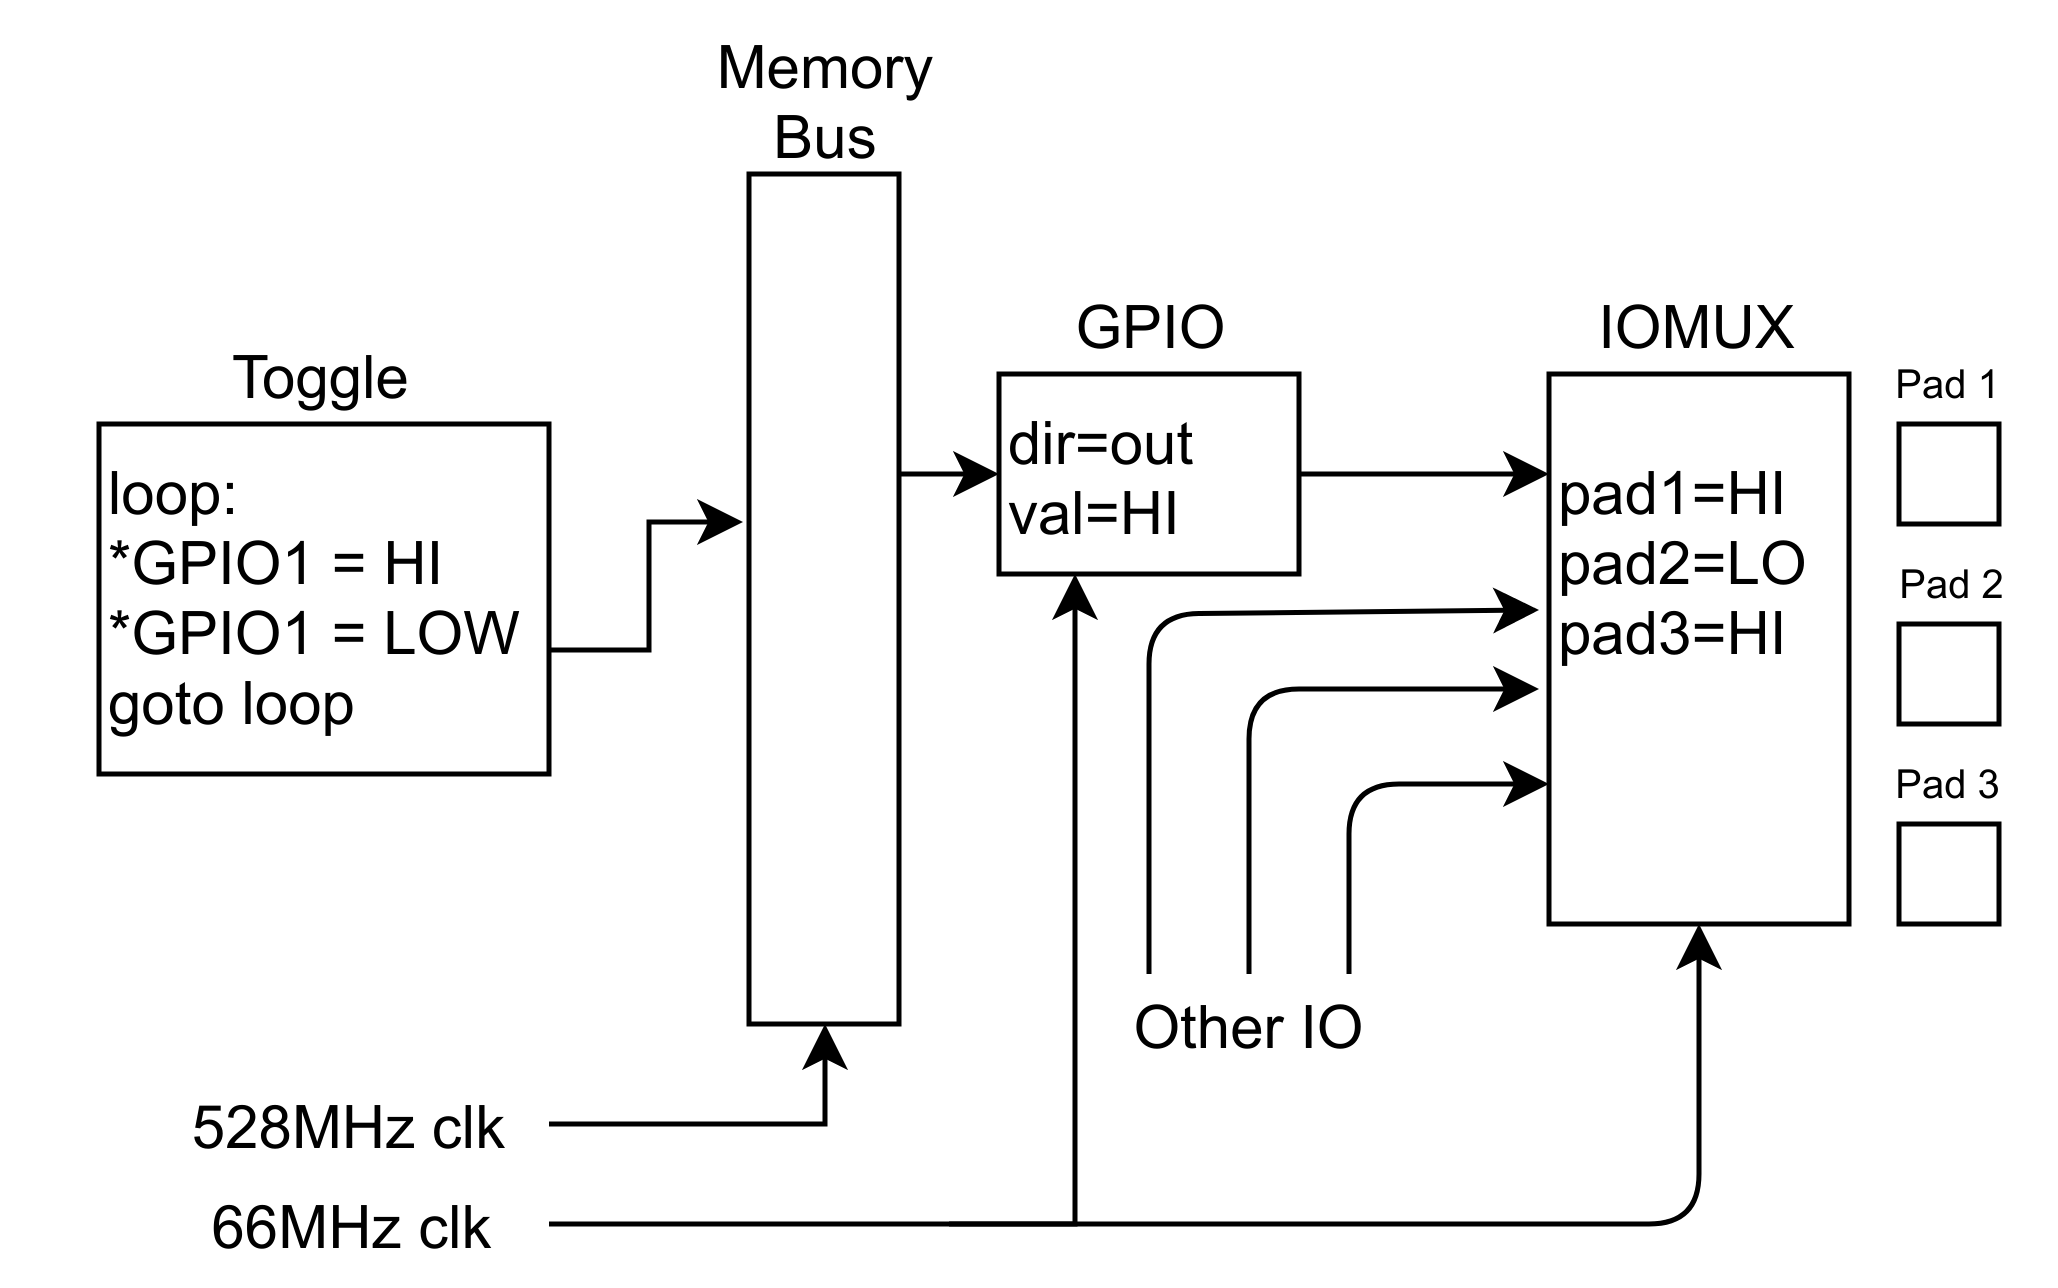
\includegraphics[scale=0.1]{pipeline}
\end{center}
  \caption{iMX6 Peripheral Latency} \label{fig:pipeline}
\end{figure}

In ARM assembly, pin toggle can be implemented in 4 lines, but compilers and 
abstractions can increase the instruction count. Higher pin
toggling frequency indicates less code in the critical path.
GERT toggles the GPIO pin by directly interfacing with the GPIO
peripheral on the iMX6, but userspace Linux code must use the
sysfs driver.
Results are shown in figure \ref{fig:toggle}.


\begin{figure} [h]
\begin{center}
  \begin{tabular}{ | l | l |}
    \hline
    Platform & Avg GPIO Toggle Rate \\ \hline
    ASM & 1.65MHz \\ \hline
    GERT Static & 568KHz \\ \hline
    Linux C & 263KHz \\ \hline
    GERT & 154KHz \\ \hline
    Linux Go & 127KHz \\
    \hline
  \end{tabular}
\end{center}
  \caption{GPIO Toggle Rates of Different Platforms}  \label{fig:toggle}
\end{figure}

%%The results show that GERT does suffer a performance decrease because of
%%Go's abstraction cost but it is not clear why GERT underperforms user-space
%%Linux C code.
%%Without all of the syscalls a user-space program must endure, there should have
%%been a speed increase.

The results of the pin toggle initially show that GERT under performs compared to
user-space Linux C. The reason became clear after tracing GERT's execution in QEMU:
the slowdown is caused by Go's interfaces in the embedded package. The GPIO driver
in the embedded package uses Go interfaces to abstract all of the different pins.
In order to toggle a single pin with an interface requires 47 instructions:
2 function calls, 19 loads, and 11 stores. In order to increase the toggle speed,
a new static GPIO driver was developed for GERT. The new driver is just a thin layer
over the memory-mapped registers. With static device ID's, the toggled pin
can be inferred at compile time instead of run time.
The performance of the static driver is also shown in the GERT static row
of figure \ref{fig:toggle}. With a static driver, GERT is able to toggle a
pin faster than user-space C code, but it is slower compared to
assembly.

%%But what if a Linux kernel module toggled the pin instead of userland code?
%%Pin toggle from inside a kernel module would certainly be faster than userland
%%C and it would also likely be faster than GERT. Operating from within
%%kernel space is very dangerous though because it lacks the protections that
%%GERT and userspace have.

\subsection{Response Latency}\label{sec:int_time}
This test measures the time it takes GERT to respond to an external event
with another external event. Specifically, it is the time it takes to produce
a rising edge on a GPIO pin in response to a falling edge on a different GPIO pin.
Faster response times are important for real time control systems, such as ABS brakes
in a car or medical equipment.
GERT and the Teensy detect the event with hardware interrupts
but Linux polls the input pin in a tight loop because the userspace sysfs
driver does not expose interrupt attachment points.
Results are shown below in figure \ref{fig:RT}.

\begin{figure} [h]
\begin{center}
  \begin{tabular}{ | l | l |}
    \hline
    Platform & Event Reponse Time \\ \hline
    Teensy 3.2 & 1$\mu$s \\ \hline
    GERT & 6.3$\mu$s \\ \hline
    Linux C & 10$\mu$s \\ \hline
    Linux Go & 30$\mu$s \\
    \hline
  \end{tabular}
\end{center}
  \caption{Event Response Times of Different Platforms}  \label{fig:RT}
\end{figure}

The event response times follow the increasing abstraction cost for each system.
The Teensy is very fast because its interrupt controller is vectored and interrupts
do not cause a stack switch. This means that the Teensy can flip a pin within a few cycles
of receiving the interrupt. GERT is slower because the iMX6 does not have a
vectored interrupt controller, the interrupt stack must be switched, and the
interrupt handler is written in Go. When GERT gets an interrupt, it must save its
current state, decide which interrupt it received, and execute its Go handler. Despite this
complexity, the iMX6 can execute more instructions in less time because of its very
high clock rate (792MHz vs 96MHz) so it can keep up with the Teensy.

The Linux configuration is slower because external interrupts cannot directly trigger a response
from userspace. In Linux, the GPIO pins are represented by file descriptors so
IO is performed by reading/writing from the appropriate file. In response to an external interrupt,
the Linux kernel sets a flag on the file descriptor which means that there is data to read. The userspace
program does not actually see the data until it is scheduled again.

\subsection{External Event Throughput} \label{sec:thruput}
Embedded systems sometimes have to monitor multiple sources of external events
whose frequencies exceed the capabilities of a single cpu. In this situation,
additional CPU's must be dedicated for the embedded system to reach its throughput
target. This benchmark attempts to simulate such a scenario by delivering a clock
signal simultaneously to 4 external GPIO pins on the iMX6. The total event throughput
should be $n \cdot frequency$ where $n$ is the number of GPIO pins being monitored and
$frequency$ is the input clock frequency. The frequency of the clock is
increased until each platform starts producing incorrect count totals.

Unfortunately, due to the semantics of the ARM Generic Interrupt Controller and the implications of its 1-N model,
it is not possible to dedicate
multiple CPU's to a single interrupt without also having expensive program logic in the interrupt handler to ensure that
only one CPU can service the interrupt. Additionally, this concept does not even exist in Linux userspace
because the state of each pin is represented as a file descriptor and concurrent reads are undefined for file descriptors.
Instead, this test program dedicates one additional CPU for each event that must be processed, up to four CPU's and events.
Doing this is easy in GERT because the target CPU of an interrupt event can be specified during attachment.
In Linux, this is accomplished by dedicating each open file descriptor to a single reader thread.

The purpose of this benchmark is to observe how the total number of serviceable external events can scale
with the number of dedicated CPU's. The results for each platform platform are shown in fig. \ref{fig:thrugraph}.

\begin{figure}[h]
\begin{center}
  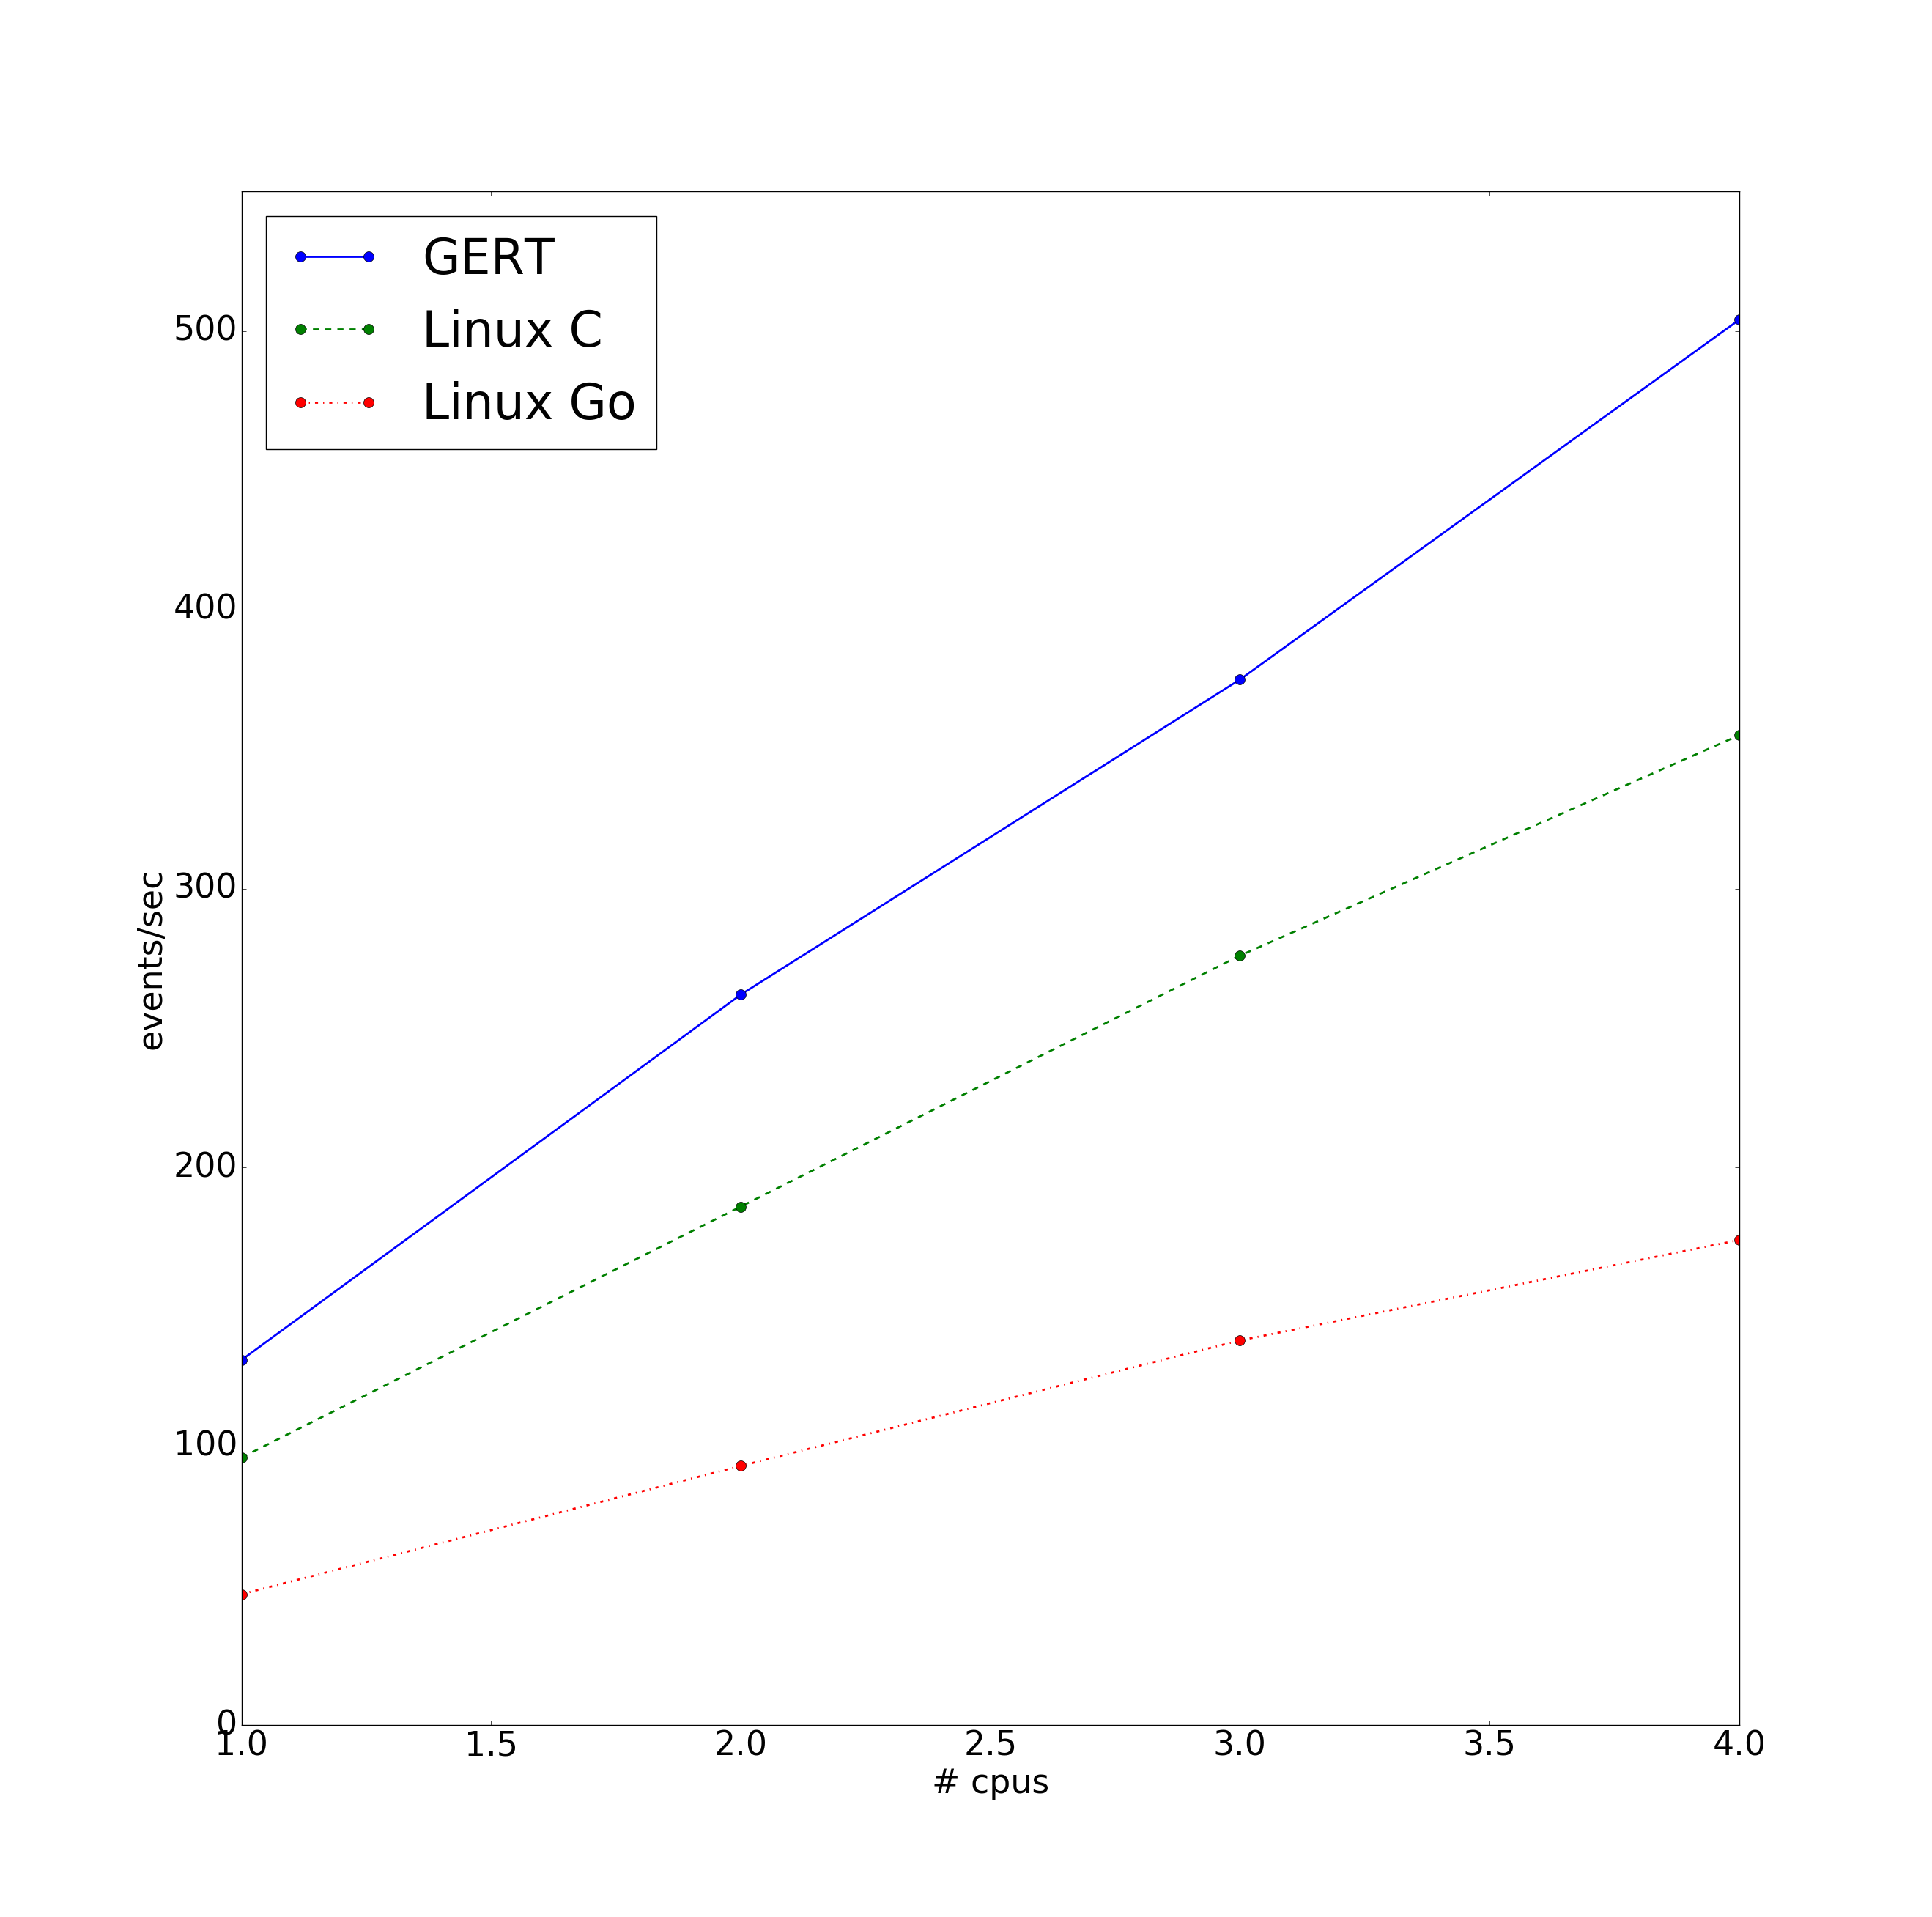
\includegraphics[scale=0.2]{throughput}
\end{center}
  \caption{Platform Event Throughput as CPU's and Events Increase} \label{fig:thrugraph}
\end{figure}

The event throughput of every platform scales approximately linearly, with GERT achieving
the highest throughput. This is an unsurprising result again because Linux file descriptors
are slower at delivering events than a true interrupt handler. GERT's higher event throughput per
core means that potentially fewer CPU's can be used to process the same amount of events. This reduces
power and space requirements.

%%Events can occur at a high enough rate such that the monitoring must
%%be spread apart on different cpus. In these kinds of applications, higher interrupt
%%throughput is a desireable property.
%%
%%\section{Pulse Counting}\label{sec:pulse_count}
%%This test measures GERT's ability to count incoming pulses. Missed pulses
%%indicate an excessively long interrupt handler that is still executing when the next
%%pulse arrives. None of the platforms were configured for re-entrant interrupt handlers
%%so they can all potentially miss pulses.
%%
%%A Xilinx Artix 7 FPGA provides ten pulses to each platform at increasing frequencies
%%until each platform misses a single pulse. The Linux benchmarks are run with polling
%%again because the
%%userspace sysfs driver does not support interrupt attachment.
%%Results are shown in figure \ref{fig:counter}.
%%
%%
%%\begin{figure} [h]
%%\begin{center}
%%  \begin{tabular}{ | l | l | l | l |}
%%    \hline
%%    Platform & Max Pulse Rate \\ \hline
%%    Teensy 3.2 & 2.50MHz\\ \hline
%%    GERT & 161KHz\\ \hline
%%    Linux C & 149KHz\\ \hline
%%    Linux Go & 84KHz\\
%%    \hline
%%  \end{tabular}
%%\end{center}
%%  \caption{Pulse Counts of Different Platforms}  \label{fig:counter}
%%\end{figure}
%%
%%GERT and userspace Linux C achieve similar performance on this test.
%%Linux just missed a few pulses.
%%
%%The Teensy registers more pulses than any other platform because of its
%%compact and efficient architecture. A dissassembly of the Cortex M4 pulse count binary
%%reveals a fully vectorized interrupt whose routine only contains 5
%%instructions and zero conditional statements.
%%
%%\section{Concurrent Events}\label{sec:concurrency}
%%Since the iMX6 has 4 cores, GERT should be able to concurrently
%%register 4 interrupts. In this test, the Teensy is configured to produce
%%ten rising edges at increasing frequencies. Each must platform must
%%register a total of 40 pulses concurrently. The maximum concurrent
%%pulse frequency for each platform before it starts missing pulses is shown in \ref{fig:counter}.
%%
%%%%In this test, the Teensy is configured to produce 10 rising edges
%%%%at 100KHz on a single pin and GERT must concurrently register them on 4 different
%%%%GPIO pins. The sum total of registered edges should be $10\times4=40$.
%%
%%%%Because polling is a blocking operation, a multithreaded Linux C program that concurrently
%%%%polls 4 pins is used for this test. The multithreaded C program is also compared
%%%%to a single-threaded C program. A multithreaded Go program which uses goroutines
%%%%to monitor pin states is also included.
%%%%Results are shown in figure \ref{fig:ccounter}.
%%
%%%%\begin{figure} [h]
%%%%\begin{center}
%%%%  \begin{tabular}{ | l | l | l | l | l |}
%%%%    \hline
%%%%    Platform & Pulse Count & Pulse Rate & Min Registered & Max Registered \\ \hline
%%%%    GERT & 10 & 100KHz & 36 & 42 \\ \hline
%%%%    Linux C Multithread & 10 & 100KHz & 32 & 33 \\ \hline
%%%%    Linux C & 10 & 100KHz & 9 & 13 \\ \hline
%%%%    Linux Go & 10 & 100KHz & TBD & TBD \\
%%%%    \hline
%%%%  \end{tabular}
%%%%\end{center}
%%%%  \caption{Concurrent Pulse Counts of Different Platforms}  \label{fig:ccounter}
%%%%\end{figure}
%%
%%\begin{figure} [h]
%%\begin{center}
%%  \begin{tabular}{ | l | l |}
%%    \hline
%%    Platform & Pulse Rate \\ \hline
%%    GERT & 126KHz \\ \hline
%%    Linux C Multithread & 109KHz \\ \hline
%%    Linux Go & 75.7KHz \\
%%    \hline
%%  \end{tabular}
%%\end{center}
%%  \caption{Concurrent Pulse Counts of Different Platforms}  \label{fig:ccounter}
%%\end{figure}
%%
%%A peculiar observation is that each platform cannot register concurrent events as fast as a single
%%event. This due to the serial architecture of the ARM Generic Interrupt Controller (GIC for short).
%%The GIC is composed of two main subsystems: the interrupt distributer and multiple CPU interfaces.
%%The task of the distributor is to aggregate all pending interrupts and distribute them to each cpu
%%in a priority order. The distributor waits for the cpu interface to acknowledge the highest priority
%%interrupt before distributing the next interrupt.
%%Unfortunately, the distributor cannot concurrently distribute interrupts even if
%%each one must go to a different cpu interface. This behavior of the ARM GIC is quite disheartening
%%for ARM SOCs because, even though it allows for concurrent \textit{detection}, it does not allow for
%%concurrent processing of interrupts. The GIC's sequential nature means that interrupt handling latency
%%is linear in the number of concurrent external events and length of the interrupt handler. A quick way
%%to reduce the apparent length of the interrupt handler is to immediately acknowledge a pending interrupt
%%before it is serviced. This allows for the distributor to signal the next interrupt more quickly but it does
%%not remove the linear time constraint.
%%
%%GERT can register concurrent external events at a slightly faster frequency than a multithreaded C program.
%%Also keep in mind that all of the Linux benchmark programs must poll in a tight loop. Polling is unlikely in a
%%real-world scenario because the cpu has other work to perform. GERT uses a true interrupt handler so that cpus
%%running GERT can be pulled away from any work they're doing in order to service the interrupt.


\section{Micro benchmark Conclusions}

Despite being written in a HLL, GERT can usually outperform userspace
Linux C code in the benchmarks that were conducted. GERT's performance trailed
Linux in the GPIO toggle test but, after changing the driver to a static model,
it also beat Linux in that test too. This is a promising result because it shows
that a HLL, which provides the same isolations as an OS kernel, can run on bare metal
and achieve higher performance than a user space C program.

Unlike Linux, GERT utilizes a true interrupt handler for delivering events.
This does not seem to matter very much for event latency, but it can explain
the throughput differences between GERT and Linux. In GERT, the interrupt handler
can directly increment the event count, but in Linux the userspace program
must indirectly observe the event by reading a file descriptor. If the user space
program reads at a bad time, it can miss a few events before reading again.

%%In reality this does not seem to matter a lot because the latency difference
%%is still just a few microseconds. Unfortunately, GERT's interrupt handling
%%process requires a context switch so it is still too slow for meeting hard
%%deadlines.

GERT and Linux have similar concurrent capabilities. When the frequency of external
events exceeds the response time of a single core, the events can be split among
multiple cores. In GERT, though, this threshold frequency is about 35KHz faster
so the programmer can avoid dedicating additional cores in some cases.

The Go garbage collector was never an issue during any of the tests because the
benchmark programs were all static. Without memory to reclaim, the GC never
had to run. However, if the GC did run, the only test that would have been affected is
the pin toggle test because the GC is allowed to stop the world. In GERT, interrupts
can trigger even when the world is stopped so the GC will not affect the event latency
and throughput benchmarks, but a GC cycle will affect these benchmarks in the Linux Go
program since it polls.

\section{Case Study: Robot Sensor Platform} \label{sec:robot}

\begin{figure}[h]
\begin{center}
  \begin{tabular}{ | l | l |}
    \hline
    Type & Line Count \\ \hline
    Initialization & 23 \\ \hline
    Event Loop & 19 \\ \hline
    ADC Driver & 106 \\ \hline
    Motor Driver & 98 \\ \hline
    UART & 41 \\ \hline
    Abstractions & 20 \\
    \hline
  \end{tabular}
\end{center}
  \caption{Code Breakdown of Robot Sensor Platform} \label{fig:robot_code}
\end{figure}

In order to evaluate GERT on a realistic workload, I put it on a robot that was
donated to me from MIT's MASLAB competition. Among other things, the robot has two drive
motors with encoders and also several Sharp GP2Y0A21YK infrared distance sensors on its perimeter.
I wrote a program in Go using GERT to process all of these event sources at the same time
and operate the robot. The working robot can move and poll the distance sensors in response to user input.
It can also measure the rotation rate of its drive motors.

The code breakdown of the robot is included in fig. \ref{fig:robot_code}. The line counts include the code that must be
included in addition to the base GERT system in order to produce the functional robot program. It is all written
in Go.

\subsection{Overview}
The main body of the robot program is an event loop which waits for events coming out of an event channel (fig. \ref{fig:event_loop}).
Independent goroutines monitor each sensor and send events into the event channel. There is a
single goroutine that monitors the event channel and manipulates state in a non-blocking manner.

The robot program uses Go's higher order functions and closures in order to create a sensor polling helper function
(fig. \ref{fig:poll_func}). In this paradigm, every sensor gets its own goroutine which sends
data back into a central event loop.

The robot program also configured the GPIO library to use interrupts in order to count pulses on the encoder (fig. \ref{fig:encoder}).

\begin{figure}[!h]
  \begin{center}
\begin{lstlisting}
select {
	case event := <-event_chan:
		fmt.Printf("%v\n", event)
		switch event {
		case "p":
			val := adc.Read(0)
			fmt.Printf("adc reads %v\n", val)
		case "w":
			drive.Forward(0.2)
		case "s":
			drive.Backward(0.2)
		case "a":
			drive.TurnRight(0.2)
		case "d":
			drive.TurnLeft(0.2)
		case " ":
			drive.Stop()
		}
	}
\end{lstlisting}
\end{center}
  \caption{Robot Event Loop} \label{fig:event_loop}
\end{figure}


\begin{figure}[!h]
\begin{center}
\begin{lstlisting}
type Pollfunc func() interface{}

func Poll(f Pollfunc, period time.Duration,
sink chan interface{}) chan bool {
	kill := make(chan bool)
	go func(kill chan bool) {
		for {
			select {
			case <-kill:
				return
			default:
				if period > 0 {
					time.Sleep(period)
				}
				sink <- f() //sink is usually the event channel
			}
		}
	}(kill)
	return kill
}
\end{lstlisting}
\end{center}
  \caption{Higher Order Polling Function} \label{fig:poll_func}
\end{figure}


\begin{figure}[!h]
\begin{center}
\begin{lstlisting}
embedded.WB_JP4_10.SetInput()
embedded.WB_JP4_10.EnableIntr(embedded.INTR_FALLING)
embedded.Enable_interrupt(99, 0) //send GPIO1 interrupt to CPU0
.
//go:nosplit
//go:nowritebarrierec
func irq(irqnum uint32) {
	switch irqnum {
...
	case 99:
		inc()
		embedded.ClearIntr(1)
...
	}
}
.
func inc() {
	count += 1
}

\end{lstlisting}
\end{center}
  \caption{Encoder Interrupt} \label{fig:encoder}
\end{figure}

With these powerful set of abstractions, adding events or sensors into the event loop
is simple because only a Pollfunc() must be implemented. As an added bonus, this
GERT program is automatically concurrent because the Go and GERT schedulers will
move idle CPU's to any available goroutine. The rest of this case study explains how the sensors
are interfaced with GERT.


\subsection{PWM Motor Control}
The robot has an MDD10A motor speed controller for controlling the two drive motors. This device
expects a pulse-width modulated signal (PWM) on its input pins in order to direct power into the
motors. A PWM signal has a constant period and the signal is a logical "on" for part of the time
and "off" for the rest of the time (fig. \ref{fig:pwm}). The ratio of "on" time vs the period is called the duty cycle.
It is this percentage which the motor controller translates into a speed for the motor.

\begin{figure}[h]
\begin{center}
  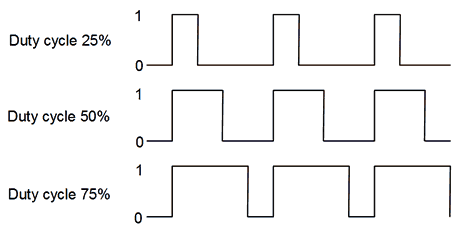
\includegraphics[scale=0.5]{pwm}
\end{center}
  \caption{Sample PWM Signals} \label{fig:pwm}
\end{figure}


The iMX6Q includes an on-board PWM peripheral which can output several channels of PWM
at a variety of periods and duty cycles. GERT contains a driver for this PWM peripheral in its embedded
package. The PWM peripheral requires no maintenance once it is configured so the cost of outputting
a PWM signal is essentially a few loads and stores every time the user changes the period or duty cycle.
The API is shown in fig. \ref{fig:pwm_api}.

The driver is organized in a typical C fashion where the memory map of the peripheral is represented in a structure (fig. \ref{fig:pwm_struct}).
Go provided little benefit for writing the driver. Even though Go is a systems language, it has poor
support for reading/writing arbitrary memory. In Go, the programmer cannot align or pad structs
and they must use the unsafe package in order to modify memory addresses with unsafe casts. This makes for a generally
unsatisfying experience when writing drivers.


\begin{figure}[h]
  \begin{subfigure}[t!]{0.5\textwidth}
  \begin{lstlisting}
  type PWM_regs struct {
	CR  uint32
	SR  uint32
	IR  uint32
	SAR uint32
	PR  uint32
	CNR uint32
}
  \end{lstlisting}
  \end{subfigure}
  \begin{subfigure}[t!]{0.5\textwidth}
 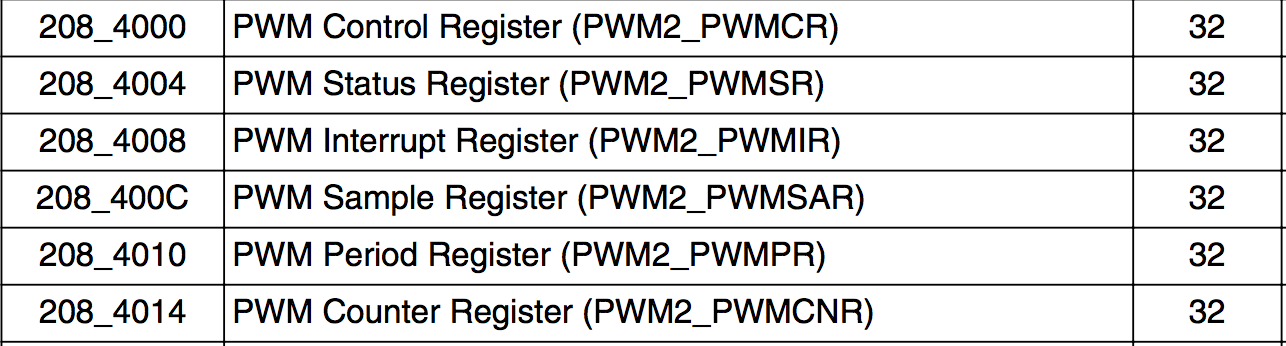
\includegraphics[scale=0.4]{pwmregs}
  \end{subfigure}
  \caption{PWM Register Representation} \label{fig:pwm_struct}
\end{figure}

\begin{figure}[h]
  \begin{lstlisting}
func (pwm *PWM_periph) Begin(freq khz)
func (pwm *PWM_periph) Stop()
func (pwm *PWM_periph) SetFreq(freq khz)
func (pwm *PWM_periph) SetDuty(dutycycle float32)
  \end{lstlisting}
  \caption{PWM Driver API} \label{fig:pwm_api}
\end{figure}

\subsection{Distance Sensor Reading}
The Sharp distance sensor outputs an analog voltage proportional to its distance from the nearest object.
A Microchip MCP3008 8-channel ADC is used to convert this voltage into a digital signal. The MCP3008 communicates in clocked
serial (SPI) with 24bit data frames so the robot program uses GERT's SPI driver (fig. \ref{fig:spi_api}). Much like the
PWM peripheral, the SPI peripheral has multiple channels that can each concurrently send and receive data. The SPI
driver also requires no input from the user except for the data to transmit and receive.

\begin{figure}[h]
  \begin{lstlisting}
  func (spi *SPI_periph) Begin(mode, freq, datalength, channel uint32)
  func (spi *SPI_periph) Send(data uint32)
  func (spi *SPI_periph) Exchange(data uint32) uint32
  \end{lstlisting}
  \caption{SPI Driver API} \label{fig:spi_api}
\end{figure}


\subsection{Encoder Reading}
The robot program also includes a motor speed monitor which uses the encoders.
Encoders emit a pulse every time the motor rotates a known amount. This amount is variable depending on the
encoder resolution. The encoders on the robot motors emit pulses at a max rate of 4KHz, corresponding to
maximum motor speed. GERT had no difficulty picking up these pulses because this frequency is far less than
the max pulse frequency in fig. \ref{fig:counter}.

The robot program asynchronously reads encoders with a special goroutine which computes the pulse difference
every second (fig. \ref{fig:speedmon}). The result is sent into the event channel.

\begin{figure}[h]
\begin{center}
\begin{lstlisting}
//count is updated by the interrupt routine
//and it is the amount of encoder pulses
go func() {
  for {
    old := count
    time.Sleep(1 * time.Second)
    new := count
    event_chan <- new - old
  }
}()
\end{lstlisting}
\end{center}
  \caption{Motor Speed Monitor} \label{fig:speedmon}
\end{figure}

\subsection{Complications}
Systems do not work perfectly, and this robot is no exception. The switching motor controller used
on this robot emits a lot of noise. The 5v noise spikes measured on the oscilloscope wreaked havoc
on the 3.3v single-ended signals that the iMX6 operates with, causing serial communication failures
and spurious interrupts. To deal with this, the robot's motors are connected to an external power supply before
taking encoder measurements in order to remove noise from the digital circuits. Consequently, the physical
robot cannot move when the motors are connected to an external power supply.

\subsection{Result}
GERT is a plausible embedded toolkit to use for robots that incorporate many sensor systems.
By utilizing Go's language features, an embedded firmware engineer can implement a complicated sensor integration
platform on top of GERT without worrying about issues like scheduling or shared memory. Because it is written in Go,
the robot sensor platform
never experienced a single use-after-free, index out of range, or memory safety bug.
As an added bonus, the robot sensor platform also does not contain a single lock despite the fact that every sensor
runs in its own thread. Go channels can still cause a deadlock though if they are used incorrectly. The Go runtime
will report total deadlock when all goroutines are blocked waiting but it cannot detect partial deadlock.

The most painful part about using GERT is writing drivers. Interacting with MMIO
peripherals inherently requires unsafe writes and reads to arbitrary memory, but Go
tries very hard to stop the programmer from doing this. Successful drivers for MMIO
peripherals must defeat the type system. In the end, a GERT driver
looks like the equivalent C driver but with many more explicit casts.
If a future version of Go deprecates the unsafe package, it will be catastrophic for
GERT's current implementation.



\section{Case Study: Laser Projector}\label{sec:laser}
\begin{figure}[h]
\begin{center}
  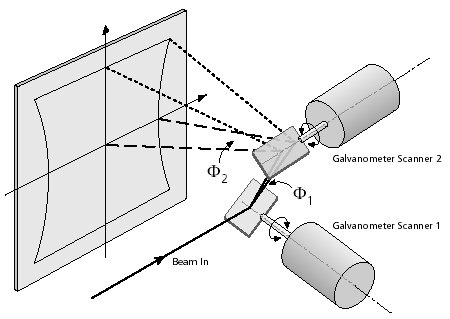
\includegraphics[scale=0.5]{galvanometer}
\end{center}
  \caption{Mirror Galvanometers} \label{fig:galvos}
\end{figure}

A scanning-mirror galvanometer laser projector is a device that deflects a laser beam off of several mirrors in
order to draw an image on another surface, as shown in fig. \ref{fig:galvos}. If the entire image can be scanned faster than 24Hz, then the light appears
to blend and the human brain perceives it as a single image rather than many points. The maximum rate at which the
projector can trace points is bounded below by the speed of the galvos and bounded above by the speed of the software.
In this case study, GERT is used to implement a laser projector with a red laser.

\subsection{Overview}
I selected a laser scanner for this case study because I have a lot of experience programming
them in C. It is interesting to observe how GERT can alter the experience.
Points for the scanner are generated from a vector graphics file on a desktop computer and stored
on an sdcard before GERT loads them and traces the image. The laser projector,
unlike the robot sensor platform, does not have to process any external events or
manage concurrency so it is a relatively simple program.

The only challenge for the laser program is to trace points fast enough so that the image appears smooth.
To do this, the laser program runs a dedicated goroutine, $lasermon$ which loops over all of the points
in a circular buffer and sends them in order to a Microchip MCP4922 DAC. The
DAC converts the digital position signal into an analog voltage and then
sends that voltage signal into an analog servo circuit, which sets the position
of the mirrors.

\subsection{Point Serialization}
The laser program uses Go's native Gob library in order to serialize and
de-serialize points. The laser projector is currently limited to
two dimensional images with a single red laser, so only three
properties must be stored for each point: X position, Y position,
and Color. The DAC only has a 12bit resolution so 16bit integers are used
to store each point. The struct is shown below in fig. \ref{fig:cpoint}

\begin{figure}[!h]
\begin{center}
\begin{lstlisting}
type CompactPoint struct {
	X     uint16
	Y     uint16
	Color uint8 //either 0 or 1
}
\end{lstlisting}
\end{center}
  \caption{Laser Point Structure} \label{fig:cpoint}
\end{figure}

In order to store points, a separate encoding program running
on a desktop computer encodes an array of $CompactPoint$ structs into
a Gob object and writes them to a file. Next, a utility called
\textit{go-bindata} is used to embed the gob file into the laser scanner
program. Then the laser scanner reads the gob'ed data during initialization.
Code is shown in \ref{fig:loadpoints}.

\begin{figure}[h]
\begin{center}
\begin{lstlisting}
var points []CompactPoint
	contents, err := Asset("bindata.gob")
	if err != nil {
		panic("bindata not found")
	}
	r := bytes.NewBuffer(contents)
	d := gob.NewDecoder(r)
	err = d.Decode(&points)
	if err != nil {
		fmt.Printf("error de-GOBing:\n")
		panic(err)
	}
\end{lstlisting}
\end{center}
  \caption{Laser Point Structure} \label{fig:loadpoints}
\end{figure}

\subsection{Path Tracing}
\textit{Lasermon} draws points by looping through a circular buffer and transmitting each point to
the DAC. If lasermon sends points too fast, then the scanner cannot keep up and it displays junk. If
lasermon sends points too slow, then the scanner does not trace the image fast enough and it does not
look static.

\textit{Lasermon} attempts to mitigate these issues by heuristically adjusting how long it should wait between
sending successive points to the scanner. If the norm-2 distance of the current point is far from the last
point, \textit{lasermon} waits longer in a busy loop before transmitting the next point. With tuning, this approach can
work for a specific image, but it does not
work very well in general because the laser scanners are not an LTI system. A better solution to the scanner problem
is a state-space feedback controller which includes \textit{lasermon} in the loop. That work is out of scope for
this thesis though.

\subsection{Result}
\begin{figure}[h]
  \begin{subfigure}[t!]{0.5\textwidth}
 
\includegraphics[scale=0.4]{csail}
  \end{subfigure}
  \begin{subfigure}[t!]{0.5\textwidth}
 
\includegraphics[scale=0.4]{csail}
  \end{subfigure}
  \caption{CSAIL Logo Generated vs Traced} \label{fig:trace_v_reality}
\end{figure}
The laser scanner programmed with GERT is able to successfully trace an SVG of the CSAIL logo
at 24Hz (fig \ref{fig:trace_v_reality}). The scan rate is not a limitation of GERT, but the mirror galvos themselves. GERT is
capable of transmitting points at several megaherts --- the rate of its SPI peripheral --- but the galvos
cannot keep up with it.

The laser scanner takes no user input or external event input so it is not a very complicated program.
The most useful feature of Go, for the laser scanner, is the Gob library for point serialization.
Based on my experience programming other laser scanners in C and 8051 assembly, this one was much easier to implement because
Go caught every out-of-bounds index error and also prevented memory use errors from ever occurring.

\section{Evaluation Summary}
GERT was evaluated both quantitatively in the benchmark section and qualitatively in the case study section.
The benchmarks show that GERT can achieve lower event latency and higher event throughput than the equivalent
programs written in user space C and Go code. This is a great result because it indicates that any embedded programs
which are written for user space can achieve potentially higher performance in GERT.

Writing embedded programs in GERT is also easier than writing them in C. Channels
and goroutines are excellent concurrency primitives. With these two primitives, program architecture can be very moduler
and performant. A good example is the sensor paradigm from the Robot Sensor Platform (\ref{sec:robot}) where each
sensor became associated with a goroutine and a channel. Since GERT inherits the Go standard libraries, GERT programs
are also more portable than bare-metal C programs. If GERT ever gets ported to different platforms, existing applications
will need few modifications to run on the new platform because the Go runtime presents the same abstractions everywhere
that it runs.

